\documentclass{article}
\usepackage[margin=1in]{geometry}
\usepackage{tikz}
\usepackage{amsmath,amssymb,amstext}

\begin{document}
{\large\bf Puzzles Day One}\hfill Name: \underline{\hspace{2in}} \\

Talk about these mathematical puzzles with a nieghbor or in a small group. If
you are struggling, ask those around you. 

\textbf{Watermelons:}\footnote{Taken from \textit{Mathematical Puzzles} by Peter Winkler} Yesterday a thousand pounds of watermelons lay in the 
watermelon patch. They were 99\% water, but overnight they lost moisture to 
evaporation and now they are only 98\% water. How much do they weigh now?
(Hint: since we don't know how many pounds of water there is to start, it may
help to use a variable to represent that quantity, say $w$. What is the initial
value of $w$?)

\vfill

\textbf{Bridge Crossing:}\footnote{Taken from
www.math.utah.edu/\textasciitilde cherk/puzzles.html} A group of four people has to cross a bridge. It 
is dark, and they have to light the path with a flashlight. No more than 
two people can cross the bridge simultaneously, and the group has only one 
flashlight. It takes different time for the people in the group to cross 
the bridge: 
\begin{itemize}
\item Annie crosses the bridge in 1 minute,
\item Bob crosses the bridge in 2 minutes,
\item Charlie crosses the bridge in 5 minutes,
\item Dorothy crosses the bridge in 10 minutes. 
\end{itemize}
How can the entire group reach the other side of the bridge in 17 minutes? (They
cannot meet each other half way, throw the flashlight, etc.)

\vfill\newpage

\begin{minipage}[t]{.45\textwidth}
\vspace{0pt}
\textbf{Mountain Ranges:} There are exactly 5 mountain ranges of length 3 (these
are shown to the right, 3 refers to the length of the base).
How many mountains of length 4 are there? What if valleys are allowed? 
\end{minipage}%
\begin{minipage}[t]{0.45\textwidth}
\vspace{0pt}
\begin{center}
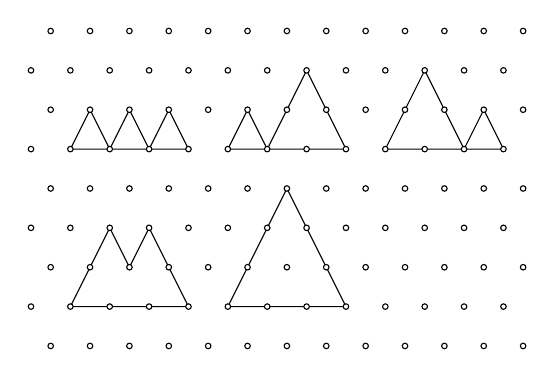
\begin{tikzpicture}[scale=0.5]

\begin{scope}[shift={(0,4)}]
\draw (0,0) -- ++(0.5,1) -- ++(0.5,-1) -- ++(0.5,1) -- ++(0.5,-1)-- ++(0.5,1) --
++(0.5,-1) -- (0,0);
\end{scope}

\begin{scope}[shift={(4,4)}]
\draw (0,0) -- ++(0.5,1) -- ++(0.5,-1) -- ++(0.5,1) -- ++(0.5,1)-- ++(0.5,-1) --
++(0.5,-1) -- (0,0);
\end{scope}
\begin{scope}[shift={(8,4)}]
\draw (0,0) -- ++(0.5,1) -- ++(0.5,1) -- ++(0.5,-1) -- ++(0.5,-1)-- ++(0.5,1) --
++(0.5,-1) -- (0,0);
\end{scope}
\begin{scope}[shift={(0,0)}]
\draw (0,0) -- ++(0.5,1) -- ++(0.5,1) -- ++(0.5,-1) -- ++(0.5,1)-- ++(0.5,-1) --
++(0.5,-1) -- (0,0);
\end{scope}
\begin{scope}[shift={(4,0)}]
\draw (0,0) -- ++(0.5,1) -- ++(0.5,1) -- ++(0.5,1) -- ++(0.5,-1)-- ++(0.5,-1) --
++(0.5,-1) -- (0,0);
\end{scope}
\foreach \x in {-1,0,1,2,3,4,5,6,7,8,9,10,11} {
    \foreach \y in {0,2,4,6} {
        \draw[fill=white] (\x,\y) circle (2pt);
    }
    \foreach \y in {-1,1,3,5,7} {
        \draw[fill=white] (\x+0.5,\y) circle (2pt);
    }
}
\end{tikzpicture}
\end{center}
\end{minipage}
\vfill


\begin{tikzpicture}[scale=0.5]
\foreach \x in {-1,0,1,2,3,4,5,6,7,8,9,10,11,12,13,14,15,16,17,18,19,20} {
    \foreach \y in {0,2,4,6,8,10,12,14,16} {
        \draw[fill=white] (\x,\y) circle (2pt);
    }
    \foreach \y in {-1,1,3,5,7,9,11,13,15,17} {
        \draw[fill=white] (\x+0.5,\y) circle (2pt);
    }
}
\end{tikzpicture}
\vfill

\end{document}
